%-*-latex-*-
\sectionthree{Hash tables}
\begin{python0}
from solutions import *; clear()
\end{python0}

A hash table (aka unordered associative array)
is very easy to understand, at least for the simple case.
Suppose we have an collection of name-height data that I want to 
keep in a container for later searching (for instance).
\begin{longtable}{|c|c|}
\hline
Name & Height \\
\hline
Abe &  6.5 \\
Tom &  5.5 \\
Annie &  5.9 \\
\hline
\end{longtable}
The key in this case is the name (of course).
The idea that I'm going to talk about has nothing to do with
name-height.
In general, it works for any so--called key-value table.
I'm going to call the above collection (vaguely) 
\defone{key--value pairs}.

Now if you think about an array, you can quickly
associate values with index values:
\begin{longtable}{|c|c|}
\hline
Index & Height \\
\hline
0 &  6.5 \\
1 &  5.5 \\
2 &  5.9 \\
\hline
\end{longtable}
The problem of course is that I have names and not index values!
Of course I can have another array of names to tie Abe, Annie, Tom to
index values:
\begin{longtable}{|c|c|}
\hline
Index & Name \\
\hline
0 &  Abe \\
1 &  Tom \\
2 &  Annie \\
\hline
\end{longtable}
But that's a pain.
Why? 
Because if you want to search for Annie's height, you
would have to search the name array to see that Annie's index is 1,
and \textit{then} go to the height array to find Annie's height.
If you add another name to the name array, then you might need
some kind of organization for fast searching.
You might think: \lq\lq Hey ... let's sort the name array!''
The problem is that the index values will then change and I 
would have to change the height array.
Bad idea!

Another way is to \textit{somehow} associate names to 
index values using some kind of numeric function.
In fact, you should know that the characters of the names
are already associated with integer values: they have ASCII codes.
For instance \verb!A! has ASCII value of 65.
Try this C/C++ statement:
\begin{console}
std::cout << int('A') << '\n';
\end{console}
They have been around for a long time: the ASCII codes were
designed by IEEE in 1960s.
So if I take inspiration from the base 10 representation of 
integers, 
I can do this to convert Abe to an integer:
\[
\text{Abe}
\rightarrow
\operatorname{int}(\texttt{A}) \cdot 10^0 +
\operatorname{int}(\texttt{b}) \cdot 10^1 +
\operatorname{int}(\texttt{e}) \cdot 10^2
\]
where $\operatorname{int}$ means the ASCII value of the relevant character.
The value you get is
%-*-latex-*-
{\footnotesize \begin{Verbatim}[frame=single,fontsize=\small]
[student@localhost discrete-probability] python tossfaircoin1.py
experiment 0 ... outcome: HEAD
experiment 1 ... outcome: TAIL
experiment 2 ... outcome: HEAD
experiment 3 ... outcome: TAIL
experiment 4 ... outcome: HEAD
experiment 5 ... outcome: TAIL
experiment 6 ... outcome: TAIL
experiment 7 ... outcome: TAIL
experiment 8 ... outcome: TAIL
experiment 9 ... outcome: TAIL
experiment 10 ... outcome: TAIL
experiment 11 ... outcome: HEAD
experiment 12 ... outcome: HEAD
experiment 13 ... outcome: TAIL
experiment 14 ... outcome: HEAD
experiment 15 ... outcome: HEAD
experiment 16 ... outcome: HEAD
experiment 17 ... outcome: TAIL
experiment 18 ... outcome: TAIL
experiment 19 ... outcome: HEAD
\end{Verbatim}
}

Now what I'm going to do is to create an array of name-height values, say that
array has size 10.
The index values are of course from 0 to 9.
No problem: the above index value, I just do mod 10 and this will give me an integer
value from 0 to 9. Right?
This means that the name \verb!Abe! will be associated with index 

\begin{center}
\begin{tikzpicture}[>=triangle 60,shorten >=0.5pt,node distance=2cm,auto,initial text=, double distance=2pt]
\node[state,initial] (A) at (  0,  0) {$\{q_0\}$};
\node[state] (B) at (  3,  0) {$\{\}$};

\path[->]
(A) edge [bend left=0,pos=0.5,above] node {$a$} (B)

;
\end{tikzpicture}
\end{center}
    


Such a function that takes data and produce an integer value 
is a hash function.
A hash function of course has a finite range.
In our case, it's from 0 to 9.
(You'll see later that frequently, you want to have the option of 
expanding the range.)
Because we're associating names to index values 0 to 9, we of course
want to make sure that names go to different index values.
Clearly with only 10 rows in your array, you cannot avoid 
hashing names to the same index values, especially if you're looking at 1000 names!
But say you have only three names.
Clearly you do want the three names to hash to different index values.
You'll see that a good quality that we want for hash functions
is that they should \lq\lq randomly scatter'' values in the range that they 
can handle. 

First let me put Abe and his height into our array, or hash table.
The above has hash function hashes Abe to 5.
So the array looks like this:

\begin{center}
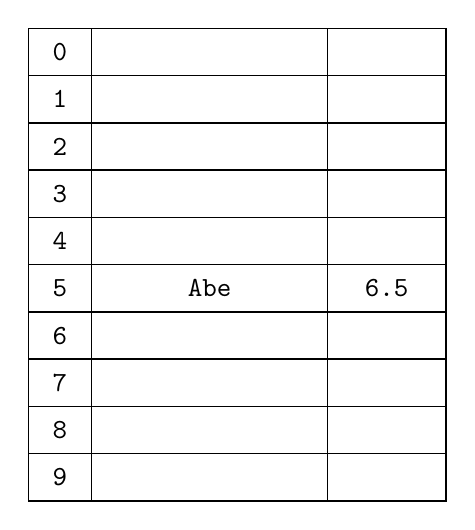
\begin{tikzpicture}

\draw (1.4, 0.7)
  node[draw, line width=0.02cm, , color=black,
       rounded corners=0cm, inner sep=0cm] {

\begin{minipage}[t][0.6cm]{0.8cm}
\mbox{}

\end{minipage}

};\draw (1.4, 0.7) node[color=black] {{\texttt{0}}};
\draw (3.3, 0.7)
  node[draw, line width=0.02cm, , color=black,
       rounded corners=0cm, inner sep=0cm] {

\begin{minipage}[t][0.6cm]{3.0cm}
\mbox{}

\end{minipage}

};\draw (3.3, 0.7) node[color=black] {{\texttt{}}};
\draw (5.55, 0.7)
  node[draw, line width=0.02cm, , color=black,
       rounded corners=0cm, inner sep=0cm] {

\begin{minipage}[t][0.6cm]{1.5cm}
\mbox{}

\end{minipage}

};\draw (5.55, 0.7) node[color=black] {{\texttt{}}};
\draw (1.4, 0.09999999999999987)
  node[draw, line width=0.02cm, , color=black,
       rounded corners=0cm, inner sep=0cm] {

\begin{minipage}[t][0.6cm]{0.8cm}
\mbox{}

\end{minipage}

};\draw (1.4, 0.09999999999999987) node[color=black] {{\texttt{1}}};
\draw (3.3, 0.09999999999999987)
  node[draw, line width=0.02cm, , color=black,
       rounded corners=0cm, inner sep=0cm] {

\begin{minipage}[t][0.6cm]{3.0cm}
\mbox{}

\end{minipage}

};\draw (3.3, 0.09999999999999987) node[color=black] {{\texttt{}}};
\draw (5.55, 0.09999999999999987)
  node[draw, line width=0.02cm, , color=black,
       rounded corners=0cm, inner sep=0cm] {

\begin{minipage}[t][0.6cm]{1.5cm}
\mbox{}

\end{minipage}

};\draw (5.55, 0.09999999999999987) node[color=black] {{\texttt{}}};
\draw (1.4, -0.5000000000000002)
  node[draw, line width=0.02cm, , color=black,
       rounded corners=0cm, inner sep=0cm] {

\begin{minipage}[t][0.6cm]{0.8cm}
\mbox{}

\end{minipage}

};\draw (1.4, -0.5000000000000002) node[color=black] {{\texttt{2}}};
\draw (3.3, -0.5000000000000002)
  node[draw, line width=0.02cm, , color=black,
       rounded corners=0cm, inner sep=0cm] {

\begin{minipage}[t][0.6cm]{3.0cm}
\mbox{}

\end{minipage}

};\draw (3.3, -0.5000000000000002) node[color=black] {{\texttt{}}};
\draw (5.55, -0.5000000000000002)
  node[draw, line width=0.02cm, , color=black,
       rounded corners=0cm, inner sep=0cm] {

\begin{minipage}[t][0.6cm]{1.5cm}
\mbox{}

\end{minipage}

};\draw (5.55, -0.5000000000000002) node[color=black] {{\texttt{}}};
\draw (1.4, -1.1000000000000003)
  node[draw, line width=0.02cm, , color=black,
       rounded corners=0cm, inner sep=0cm] {

\begin{minipage}[t][0.6cm]{0.8cm}
\mbox{}

\end{minipage}

};\draw (1.4, -1.1000000000000003) node[color=black] {{\texttt{3}}};
\draw (3.3, -1.1000000000000003)
  node[draw, line width=0.02cm, , color=black,
       rounded corners=0cm, inner sep=0cm] {

\begin{minipage}[t][0.6cm]{3.0cm}
\mbox{}

\end{minipage}

};\draw (3.3, -1.1000000000000003) node[color=black] {{\texttt{}}};
\draw (5.55, -1.1000000000000003)
  node[draw, line width=0.02cm, , color=black,
       rounded corners=0cm, inner sep=0cm] {

\begin{minipage}[t][0.6cm]{1.5cm}
\mbox{}

\end{minipage}

};\draw (5.55, -1.1000000000000003) node[color=black] {{\texttt{}}};
\draw (1.4, -1.7000000000000002)
  node[draw, line width=0.02cm, , color=black,
       rounded corners=0cm, inner sep=0cm] {

\begin{minipage}[t][0.6cm]{0.8cm}
\mbox{}

\end{minipage}

};\draw (1.4, -1.7000000000000002) node[color=black] {{\texttt{4}}};
\draw (3.3, -1.7000000000000002)
  node[draw, line width=0.02cm, , color=black,
       rounded corners=0cm, inner sep=0cm] {

\begin{minipage}[t][0.6cm]{3.0cm}
\mbox{}

\end{minipage}

};\draw (3.3, -1.7000000000000002) node[color=black] {{\texttt{}}};
\draw (5.55, -1.7000000000000002)
  node[draw, line width=0.02cm, , color=black,
       rounded corners=0cm, inner sep=0cm] {

\begin{minipage}[t][0.6cm]{1.5cm}
\mbox{}

\end{minipage}

};\draw (5.55, -1.7000000000000002) node[color=black] {{\texttt{}}};
\draw (1.4, -2.3000000000000003)
  node[draw, line width=0.02cm, , color=black,
       rounded corners=0cm, inner sep=0cm] {

\begin{minipage}[t][0.6cm]{0.8cm}
\mbox{}

\end{minipage}

};\draw (1.4, -2.3000000000000003) node[color=black] {{\texttt{5}}};
\draw (3.3, -2.3000000000000003)
  node[draw, line width=0.02cm, , color=black,
       rounded corners=0cm, inner sep=0cm] {

\begin{minipage}[t][0.6cm]{3.0cm}
\mbox{}

\end{minipage}

};\draw (3.3, -2.3000000000000003) node[color=black] {{\texttt{Abe}}};
\draw (5.55, -2.3000000000000003)
  node[draw, line width=0.02cm, , color=black,
       rounded corners=0cm, inner sep=0cm] {

\begin{minipage}[t][0.6cm]{1.5cm}
\mbox{}

\end{minipage}

};\draw (5.55, -2.3000000000000003) node[color=black] {{\texttt{6.5}}};
\draw (1.4, -2.9000000000000004)
  node[draw, line width=0.02cm, , color=black,
       rounded corners=0cm, inner sep=0cm] {

\begin{minipage}[t][0.6cm]{0.8cm}
\mbox{}

\end{minipage}

};\draw (1.4, -2.9000000000000004) node[color=black] {{\texttt{6}}};
\draw (3.3, -2.9000000000000004)
  node[draw, line width=0.02cm, , color=black,
       rounded corners=0cm, inner sep=0cm] {

\begin{minipage}[t][0.6cm]{3.0cm}
\mbox{}

\end{minipage}

};\draw (3.3, -2.9000000000000004) node[color=black] {{\texttt{}}};
\draw (5.55, -2.9000000000000004)
  node[draw, line width=0.02cm, , color=black,
       rounded corners=0cm, inner sep=0cm] {

\begin{minipage}[t][0.6cm]{1.5cm}
\mbox{}

\end{minipage}

};\draw (5.55, -2.9000000000000004) node[color=black] {{\texttt{}}};
\draw (1.4, -3.500000000000001)
  node[draw, line width=0.02cm, , color=black,
       rounded corners=0cm, inner sep=0cm] {

\begin{minipage}[t][0.6cm]{0.8cm}
\mbox{}

\end{minipage}

};\draw (1.4, -3.500000000000001) node[color=black] {{\texttt{7}}};
\draw (3.3, -3.500000000000001)
  node[draw, line width=0.02cm, , color=black,
       rounded corners=0cm, inner sep=0cm] {

\begin{minipage}[t][0.6cm]{3.0cm}
\mbox{}

\end{minipage}

};\draw (3.3, -3.500000000000001) node[color=black] {{\texttt{}}};
\draw (5.55, -3.500000000000001)
  node[draw, line width=0.02cm, , color=black,
       rounded corners=0cm, inner sep=0cm] {

\begin{minipage}[t][0.6cm]{1.5cm}
\mbox{}

\end{minipage}

};\draw (5.55, -3.500000000000001) node[color=black] {{\texttt{}}};
\draw (1.4, -4.1000000000000005)
  node[draw, line width=0.02cm, , color=black,
       rounded corners=0cm, inner sep=0cm] {

\begin{minipage}[t][0.6cm]{0.8cm}
\mbox{}

\end{minipage}

};\draw (1.4, -4.1000000000000005) node[color=black] {{\texttt{8}}};
\draw (3.3, -4.1000000000000005)
  node[draw, line width=0.02cm, , color=black,
       rounded corners=0cm, inner sep=0cm] {

\begin{minipage}[t][0.6cm]{3.0cm}
\mbox{}

\end{minipage}

};\draw (3.3, -4.1000000000000005) node[color=black] {{\texttt{}}};
\draw (5.55, -4.1000000000000005)
  node[draw, line width=0.02cm, , color=black,
       rounded corners=0cm, inner sep=0cm] {

\begin{minipage}[t][0.6cm]{1.5cm}
\mbox{}

\end{minipage}

};\draw (5.55, -4.1000000000000005) node[color=black] {{\texttt{}}};
\draw (1.4, -4.7)
  node[draw, line width=0.02cm, , color=black,
       rounded corners=0cm, inner sep=0cm] {

\begin{minipage}[t][0.6cm]{0.8cm}
\mbox{}

\end{minipage}

};\draw (1.4, -4.7) node[color=black] {{\texttt{9}}};
\draw (3.3, -4.7)
  node[draw, line width=0.02cm, , color=black,
       rounded corners=0cm, inner sep=0cm] {

\begin{minipage}[t][0.6cm]{3.0cm}
\mbox{}

\end{minipage}

};\draw (3.3, -4.7) node[color=black] {{\texttt{}}};
\draw (5.55, -4.7)
  node[draw, line width=0.02cm, , color=black,
       rounded corners=0cm, inner sep=0cm] {

\begin{minipage}[t][0.6cm]{1.5cm}
\mbox{}

\end{minipage}

};\draw (5.55, -4.7) node[color=black] {{\texttt{}}};
\end{tikzpicture}

\end{center}



(The index value is included just for convenience. Of course arrays do not contain index values.)
The C++ code would look like this:
{\small
\begin{console}
class NameHeight
{
public:
    std::string name_;
    double height_;
};

class Hashtable
{
public:
    NameHeight table_[10];
};
\end{console}
}

OK. 
Now let's put Tom into our hash table.
The hash value of Tom is
\begin{center}
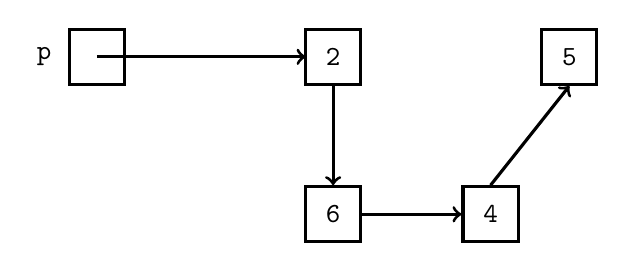
\begin{tikzpicture}

\draw (0.35, 0.35)
  node[draw, line width=0.04cm, , color=black,
       rounded corners=0cm, inner sep=0cm] {

\begin{minipage}[t][0.7cm]{0.7cm}
\mbox{}

\end{minipage}

};\draw (0.35, 0.35) node[color=black] {{\texttt{2}}};
\draw (0.35, -1.65)
  node[draw, line width=0.04cm, , color=black,
       rounded corners=0cm, inner sep=0cm] {

\begin{minipage}[t][0.7cm]{0.7cm}
\mbox{}

\end{minipage}

};\draw (0.35, -1.65) node[color=black] {{\texttt{6}}};
\draw (2.35, -1.65)
  node[draw, line width=0.04cm, , color=black,
       rounded corners=0cm, inner sep=0cm] {

\begin{minipage}[t][0.7cm]{0.7cm}
\mbox{}

\end{minipage}

};\draw (2.35, -1.65) node[color=black] {{\texttt{4}}};
\draw (3.35, 0.35)
  node[draw, line width=0.04cm, , color=black,
       rounded corners=0cm, inner sep=0cm] {

\begin{minipage}[t][0.7cm]{0.7cm}
\mbox{}

\end{minipage}

};\draw (3.35, 0.35) node[color=black] {{\texttt{5}}};\draw[line width=0.04cm,black,->] (0.35,-0.02) to  (0.35,-1.28);
\draw[line width=0.04cm,black,->] (0.72,-1.65) to  (1.98,-1.65);
\draw[line width=0.04cm,black,->] (2.35,-1.28) to  (3.35,-0.02);

\draw (-2.65, 0.35)
  node[draw, line width=0.04cm, , color=black,
       rounded corners=0cm, inner sep=0cm] {

\begin{minipage}[t][0.7cm]{0.7cm}
\mbox{}

\end{minipage}

};\draw (-2.65, 0.35) node[color=black] {{\texttt{}}};\draw[line width=0.04cm,black,->] (-2.65,0.35) to  (0,0.35);

\draw (-3.32, 0.35)
  node[draw, line width=0.04cm, , color=white,
       rounded corners=0cm, inner sep=0cm] {

\begin{minipage}[t][0.1cm]{0.1cm}
\mbox{}

\end{minipage}

};\draw (-3.32, 0.35) node[color=black] {{\texttt{p}}};
\end{tikzpicture}

\end{center}


and when I take mod 10, I get 4.

\begin{center}
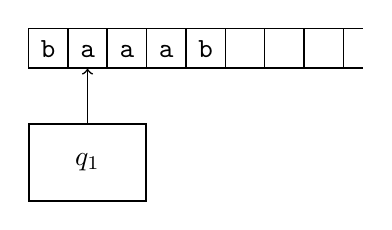
\begin{tikzpicture}

\draw (0.25, 0.25)
  node[draw, line width=0.02cm, , color=black,
       rounded corners=0cm, inner sep=0cm] {

\begin{minipage}[t][0.5cm]{0.5cm}
\mbox{}

\end{minipage}

};\draw (0.25, 0.25) node[color=black] {{\vphantom{baaab\SPACE\SPACE\SPACE}\texttt{b}}};
\draw (0.75, 0.25)
  node[draw, line width=0.02cm, , color=black,
       rounded corners=0cm, inner sep=0cm] {

\begin{minipage}[t][0.5cm]{0.5cm}
\mbox{}

\end{minipage}

};\draw (0.75, 0.25) node[color=black] {{\vphantom{baaab\SPACE\SPACE\SPACE}\texttt{a}}};
\draw (1.25, 0.25)
  node[draw, line width=0.02cm, , color=black,
       rounded corners=0cm, inner sep=0cm] {

\begin{minipage}[t][0.5cm]{0.5cm}
\mbox{}

\end{minipage}

};\draw (1.25, 0.25) node[color=black] {{\vphantom{baaab\SPACE\SPACE\SPACE}\texttt{a}}};
\draw (1.75, 0.25)
  node[draw, line width=0.02cm, , color=black,
       rounded corners=0cm, inner sep=0cm] {

\begin{minipage}[t][0.5cm]{0.5cm}
\mbox{}

\end{minipage}

};\draw (1.75, 0.25) node[color=black] {{\vphantom{baaab\SPACE\SPACE\SPACE}\texttt{a}}};
\draw (2.25, 0.25)
  node[draw, line width=0.02cm, , color=black,
       rounded corners=0cm, inner sep=0cm] {

\begin{minipage}[t][0.5cm]{0.5cm}
\mbox{}

\end{minipage}

};\draw (2.25, 0.25) node[color=black] {{\vphantom{baaab\SPACE\SPACE\SPACE}\texttt{b}}};
\draw (2.75, 0.25)
  node[draw, line width=0.02cm, , color=black,
       rounded corners=0cm, inner sep=0cm] {

\begin{minipage}[t][0.5cm]{0.5cm}
\mbox{}

\end{minipage}

};\draw (2.75, 0.25) node[color=black] {{\vphantom{baaab\SPACE\SPACE\SPACE}\texttt{\SPACE}}};
\draw (3.25, 0.25)
  node[draw, line width=0.02cm, , color=black,
       rounded corners=0cm, inner sep=0cm] {

\begin{minipage}[t][0.5cm]{0.5cm}
\mbox{}

\end{minipage}

};\draw (3.25, 0.25) node[color=black] {{\vphantom{baaab\SPACE\SPACE\SPACE}\texttt{\SPACE}}};
\draw (3.75, 0.25)
  node[draw, line width=0.02cm, , color=black,
       rounded corners=0cm, inner sep=0cm] {

\begin{minipage}[t][0.5cm]{0.5cm}
\mbox{}

\end{minipage}

};\draw (3.75, 0.25) node[color=black] {{\vphantom{baaab\SPACE\SPACE\SPACE}\texttt{\SPACE}}};\draw[line width=0.02cm,black] (4.0,0.5) to  (4.25,0.5);
\draw[line width=0.02cm,black] (4.0,0.0) to  (4.25,0.0);

\draw (0.75, -1.2)
  node[draw, line width=0.02cm, , color=black,
       rounded corners=0cm, inner sep=0cm] {

\begin{minipage}[t][0.98cm]{1.48cm}
\mbox{}

\end{minipage}

};\draw (0.75, -1.2) node[color=black] {$q_1$};\draw[line width=0.02cm,black,->] (0.75,-0.7) to  (0.75,-0.47) to  (0.75,-0.47) to  (0.75,-0.01);
\end{tikzpicture}

\end{center}



Let's take a pause and see how 
this container help us find data.
So ... if you want to know Abe's height,
all you need to do is to use our hash function, 
compute the hash value of Abe, which would be 5,
and you find what you're looking for.
Period.
Easy, right?

If you don't allow the empty string as a name,
you can initializ the names of your 
hash table to \verb!""!.
But what if you allow the empty string
as a name?
Well you can for instance include a flag in your
\verb!NameHeight! class to indicate if there's valid data or not.
Something like this:
{\small
\begin{console}
class NameHeight
{
public:
    bool available_; // or not_available if you like
    std::string name_;
    double height_;
};

class Hashtable
{
public:
    NameHeight table_[10];
};
\end{console}
}
If so, the hash table now looks like this


\begin{center}
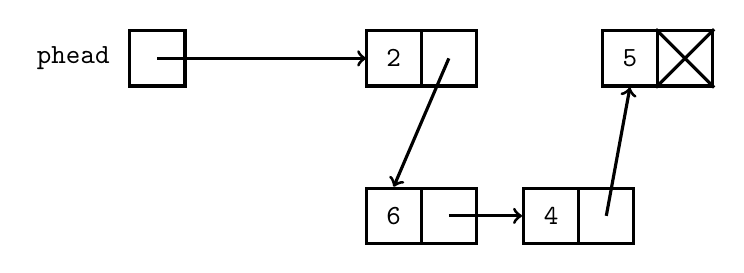
\begin{tikzpicture}

\draw (0.35, 0.35)
  node[draw, line width=0.04cm, , color=black,
       rounded corners=0cm, inner sep=0cm] {

\begin{minipage}[t][0.7cm]{0.7cm}
\mbox{}

\end{minipage}

};\draw (0.35, 0.35) node[color=black] {{\texttt{2}}};
\draw (1.0499999999999998, 0.35)
  node[draw, line width=0.04cm, , color=black,
       rounded corners=0cm, inner sep=0cm] {

\begin{minipage}[t][0.7cm]{0.7cm}
\mbox{}

\end{minipage}

};\draw (1.0499999999999998, 0.35) node[color=black] {{\texttt{}}};
\draw (0.35, -1.65)
  node[draw, line width=0.04cm, , color=black,
       rounded corners=0cm, inner sep=0cm] {

\begin{minipage}[t][0.7cm]{0.7cm}
\mbox{}

\end{minipage}

};\draw (0.35, -1.65) node[color=black] {{\texttt{6}}};
\draw (1.0499999999999998, -1.65)
  node[draw, line width=0.04cm, , color=black,
       rounded corners=0cm, inner sep=0cm] {

\begin{minipage}[t][0.7cm]{0.7cm}
\mbox{}

\end{minipage}

};\draw (1.0499999999999998, -1.65) node[color=black] {{\texttt{}}};
\draw (2.35, -1.65)
  node[draw, line width=0.04cm, , color=black,
       rounded corners=0cm, inner sep=0cm] {

\begin{minipage}[t][0.7cm]{0.7cm}
\mbox{}

\end{minipage}

};\draw (2.35, -1.65) node[color=black] {{\texttt{4}}};
\draw (3.0500000000000003, -1.65)
  node[draw, line width=0.04cm, , color=black,
       rounded corners=0cm, inner sep=0cm] {

\begin{minipage}[t][0.7cm]{0.7cm}
\mbox{}

\end{minipage}

};\draw (3.0500000000000003, -1.65) node[color=black] {{\texttt{}}};
\draw (3.35, 0.35)
  node[draw, line width=0.04cm, , color=black,
       rounded corners=0cm, inner sep=0cm] {

\begin{minipage}[t][0.7cm]{0.7cm}
\mbox{}

\end{minipage}

};\draw (3.35, 0.35) node[color=black] {{\texttt{5}}};
\draw (4.05, 0.35)
  node[draw, line width=0.04cm, , color=black,
       rounded corners=0cm, inner sep=0cm] {

\begin{minipage}[t][0.7cm]{0.7cm}
\mbox{}

\end{minipage}

};\draw (4.05, 0.35) node[color=black] {{\texttt{}}};\draw[line width=0.04cm,black,->] (1.05,0.35) to  (0.35,-1.28);
\draw[line width=0.04cm,black,->] (1.05,-1.65) to  (1.98,-1.65);
\draw[line width=0.04cm,black,->] (3.05,-1.65) to  (3.35,-0.02);
\draw[line width=0.04cm,black] (3.68,0.72) to  (4.42,-0.02);
\draw[line width=0.04cm,black] (4.42,0.72) to  (3.68,-0.02);

\draw (-2.65, 0.35)
  node[draw, line width=0.04cm, , color=black,
       rounded corners=0cm, inner sep=0cm] {

\begin{minipage}[t][0.7cm]{0.7cm}
\mbox{}

\end{minipage}

};\draw (-2.65, 0.35) node[color=black] {{\texttt{}}};\draw[line width=0.04cm,black,->] (-2.65,0.35) to  (0,0.35);

\draw (-3.7199999999999998, 0.35)
  node[draw, line width=0.04cm, , color=white,
       rounded corners=0cm, inner sep=0cm] {

\begin{minipage}[t][0.1cm]{0.1cm}
\mbox{}

\end{minipage}

};\draw (-3.7199999999999998, 0.35) node[color=black] {{\texttt{phead}}};
\end{tikzpicture}

\end{center}



It's also possible to have a hash table that contains
the keys, but the 
data can be placed in the heap, i.e.,
the hash table is an array of key-pointer values.
In that case, the hash table would take less space --
don't forget that a huge array makes memory management
difficult because the array of values must be contiguous.
And this is a good thing.

\begin{center}
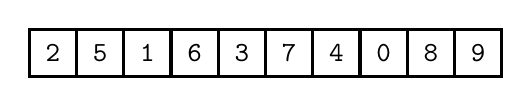
\begin{tikzpicture}

\draw (0.3, -0.3)
  node[draw, line width=0.04cm, , color=black,
       rounded corners=0cm, inner sep=0cm] {

\begin{minipage}[t][0.6cm]{0.6cm}
\mbox{}

\end{minipage}

};\draw (0.3, -0.3) node[color=black] {{\texttt{2}}};
\draw (0.8999999999999999, -0.3)
  node[draw, line width=0.04cm, , color=black,
       rounded corners=0cm, inner sep=0cm] {

\begin{minipage}[t][0.6cm]{0.6cm}
\mbox{}

\end{minipage}

};\draw (0.8999999999999999, -0.3) node[color=black] {{\texttt{5}}};
\draw (1.5, -0.3)
  node[draw, line width=0.04cm, , color=black,
       rounded corners=0cm, inner sep=0cm] {

\begin{minipage}[t][0.6cm]{0.6cm}
\mbox{}

\end{minipage}

};\draw (1.5, -0.3) node[color=black] {{\texttt{1}}};
\draw (2.0999999999999996, -0.3)
  node[draw, line width=0.04cm, , color=black,
       rounded corners=0cm, inner sep=0cm] {

\begin{minipage}[t][0.6cm]{0.6cm}
\mbox{}

\end{minipage}

};\draw (2.0999999999999996, -0.3) node[color=black] {{\texttt{6}}};
\draw (2.7, -0.3)
  node[draw, line width=0.04cm, , color=black,
       rounded corners=0cm, inner sep=0cm] {

\begin{minipage}[t][0.6cm]{0.6cm}
\mbox{}

\end{minipage}

};\draw (2.7, -0.3) node[color=black] {{\texttt{3}}};
\draw (3.3, -0.3)
  node[draw, line width=0.04cm, , color=black,
       rounded corners=0cm, inner sep=0cm] {

\begin{minipage}[t][0.6cm]{0.6cm}
\mbox{}

\end{minipage}

};\draw (3.3, -0.3) node[color=black] {{\texttt{7}}};
\draw (3.9, -0.3)
  node[draw, line width=0.04cm, , color=black,
       rounded corners=0cm, inner sep=0cm] {

\begin{minipage}[t][0.6cm]{0.6cm}
\mbox{}

\end{minipage}

};\draw (3.9, -0.3) node[color=black] {{\texttt{4}}};
\draw (4.5, -0.3)
  node[draw, line width=0.04cm, , color=black,
       rounded corners=0cm, inner sep=0cm] {

\begin{minipage}[t][0.6cm]{0.6cm}
\mbox{}

\end{minipage}

};\draw (4.5, -0.3) node[color=black] {{\texttt{0}}};
\draw (5.1, -0.3)
  node[draw, line width=0.04cm, , color=black,
       rounded corners=0cm, inner sep=0cm] {

\begin{minipage}[t][0.6cm]{0.6cm}
\mbox{}

\end{minipage}

};\draw (5.1, -0.3) node[color=black] {{\texttt{8}}};
\draw (5.699999999999999, -0.3)
  node[draw, line width=0.04cm, , color=black,
       rounded corners=0cm, inner sep=0cm] {

\begin{minipage}[t][0.6cm]{0.6cm}
\mbox{}

\end{minipage}

};\draw (5.699999999999999, -0.3) node[color=black] {{\texttt{9}}};
\end{tikzpicture}

\end{center}


In this case, we don't even need the availability flag since a
\verb!NULL! pointer would tell us that the row is available.

But ... we can take this one step further ...
another option is to have a hash table not be 
name-pointer rows,
but of pointers all altogether.
Here's what I mean (in pictures):

\begin{center}
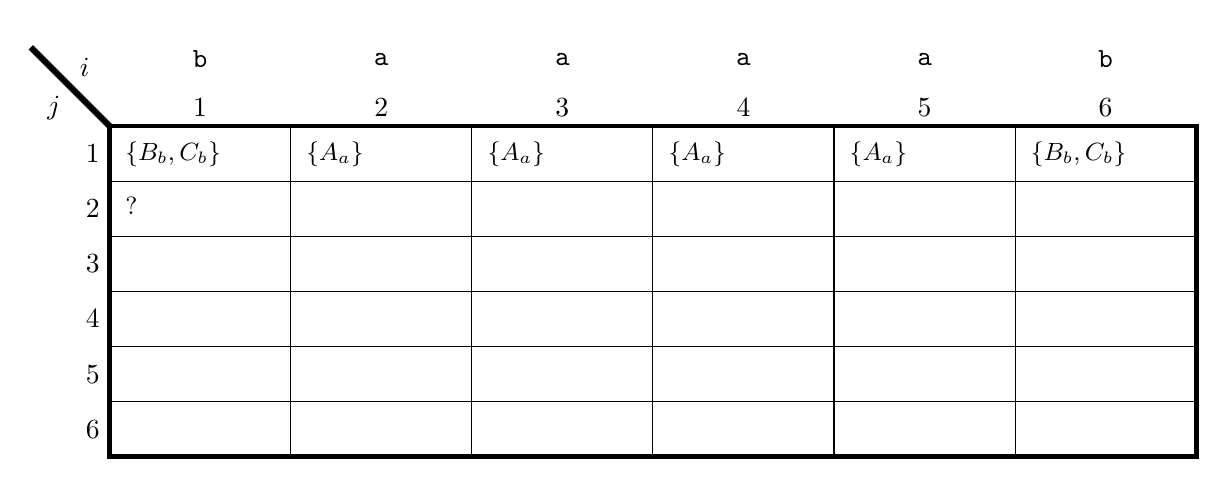
\begin{tikzpicture}

\draw (1.15, -0.35)
  node[draw, , , color=black,
       rounded corners=0cm, inner sep=0.2cm] {

\begin{minipage}[t][0.3cm]{1.9cm}
\mbox{}

\end{minipage}

};
\draw (1.15, -0.35) node[color=black,
 inner sep=0.2cm] {
 
\begin{minipage}[t][0.3cm]{1.9cm}
{\small $\{B_b,C_b\}$}
\end{minipage}

};
\draw (3.4499999999999997, -0.35)
  node[draw, , , color=black,
       rounded corners=0cm, inner sep=0.2cm] {

\begin{minipage}[t][0.3cm]{1.9cm}
\mbox{}

\end{minipage}

};
\draw (3.4499999999999997, -0.35) node[color=black,
 inner sep=0.2cm] {
 
\begin{minipage}[t][0.3cm]{1.9cm}
{\small $\{A_a\}$}
\end{minipage}

};
\draw (5.75, -0.35)
  node[draw, , , color=black,
       rounded corners=0cm, inner sep=0.2cm] {

\begin{minipage}[t][0.3cm]{1.9cm}
\mbox{}

\end{minipage}

};
\draw (5.75, -0.35) node[color=black,
 inner sep=0.2cm] {
 
\begin{minipage}[t][0.3cm]{1.9cm}
{\small $\{A_a\}$}
\end{minipage}

};
\draw (8.049999999999999, -0.35)
  node[draw, , , color=black,
       rounded corners=0cm, inner sep=0.2cm] {

\begin{minipage}[t][0.3cm]{1.9cm}
\mbox{}

\end{minipage}

};
\draw (8.049999999999999, -0.35) node[color=black,
 inner sep=0.2cm] {
 
\begin{minipage}[t][0.3cm]{1.9cm}
{\small $\{A_a\}$}
\end{minipage}

};
\draw (10.35, -0.35)
  node[draw, , , color=black,
       rounded corners=0cm, inner sep=0.2cm] {

\begin{minipage}[t][0.3cm]{1.9cm}
\mbox{}

\end{minipage}

};
\draw (10.35, -0.35) node[color=black,
 inner sep=0.2cm] {
 
\begin{minipage}[t][0.3cm]{1.9cm}
{\small $\{A_a\}$}
\end{minipage}

};
\draw (12.65, -0.35)
  node[draw, , , color=black,
       rounded corners=0cm, inner sep=0.2cm] {

\begin{minipage}[t][0.3cm]{1.9cm}
\mbox{}

\end{minipage}

};
\draw (12.65, -0.35) node[color=black,
 inner sep=0.2cm] {
 
\begin{minipage}[t][0.3cm]{1.9cm}
{\small $\{B_b,C_b\}$}
\end{minipage}

};
\draw (1.15, -1.0499999999999998)
  node[draw, , , color=black,
       rounded corners=0cm, inner sep=0.2cm] {

\begin{minipage}[t][0.3cm]{1.9cm}
\mbox{}

\end{minipage}

};
\draw (1.15, -1.0499999999999998) node[color=black,
 inner sep=0.2cm] {
 
\begin{minipage}[t][0.3cm]{1.9cm}
{\small ?}
\end{minipage}

};
\draw (3.4499999999999997, -1.0499999999999998)
  node[draw, , , color=black,
       rounded corners=0cm, inner sep=0.2cm] {

\begin{minipage}[t][0.3cm]{1.9cm}
\mbox{}

\end{minipage}

};
\draw (3.4499999999999997, -1.0499999999999998) node[color=black,
 inner sep=0.2cm] {
 
\begin{minipage}[t][0.3cm]{1.9cm}
{\small }
\end{minipage}

};
\draw (5.75, -1.0499999999999998)
  node[draw, , , color=black,
       rounded corners=0cm, inner sep=0.2cm] {

\begin{minipage}[t][0.3cm]{1.9cm}
\mbox{}

\end{minipage}

};
\draw (5.75, -1.0499999999999998) node[color=black,
 inner sep=0.2cm] {
 
\begin{minipage}[t][0.3cm]{1.9cm}
{\small }
\end{minipage}

};
\draw (8.049999999999999, -1.0499999999999998)
  node[draw, , , color=black,
       rounded corners=0cm, inner sep=0.2cm] {

\begin{minipage}[t][0.3cm]{1.9cm}
\mbox{}

\end{minipage}

};
\draw (8.049999999999999, -1.0499999999999998) node[color=black,
 inner sep=0.2cm] {
 
\begin{minipage}[t][0.3cm]{1.9cm}
{\small }
\end{minipage}

};
\draw (10.35, -1.0499999999999998)
  node[draw, , , color=black,
       rounded corners=0cm, inner sep=0.2cm] {

\begin{minipage}[t][0.3cm]{1.9cm}
\mbox{}

\end{minipage}

};
\draw (10.35, -1.0499999999999998) node[color=black,
 inner sep=0.2cm] {
 
\begin{minipage}[t][0.3cm]{1.9cm}
{\small }
\end{minipage}

};
\draw (12.65, -1.0499999999999998)
  node[draw, , , color=black,
       rounded corners=0cm, inner sep=0.2cm] {

\begin{minipage}[t][0.3cm]{1.9cm}
\mbox{}

\end{minipage}

};
\draw (12.65, -1.0499999999999998) node[color=black,
 inner sep=0.2cm] {
 
\begin{minipage}[t][0.3cm]{1.9cm}
{\small }
\end{minipage}

};
\draw (1.15, -1.7499999999999996)
  node[draw, , , color=black,
       rounded corners=0cm, inner sep=0.2cm] {

\begin{minipage}[t][0.3cm]{1.9cm}
\mbox{}

\end{minipage}

};
\draw (1.15, -1.7499999999999996) node[color=black,
 inner sep=0.2cm] {
 
\begin{minipage}[t][0.3cm]{1.9cm}
{\small }
\end{minipage}

};
\draw (3.4499999999999997, -1.7499999999999996)
  node[draw, , , color=black,
       rounded corners=0cm, inner sep=0.2cm] {

\begin{minipage}[t][0.3cm]{1.9cm}
\mbox{}

\end{minipage}

};
\draw (3.4499999999999997, -1.7499999999999996) node[color=black,
 inner sep=0.2cm] {
 
\begin{minipage}[t][0.3cm]{1.9cm}
{\small }
\end{minipage}

};
\draw (5.75, -1.7499999999999996)
  node[draw, , , color=black,
       rounded corners=0cm, inner sep=0.2cm] {

\begin{minipage}[t][0.3cm]{1.9cm}
\mbox{}

\end{minipage}

};
\draw (5.75, -1.7499999999999996) node[color=black,
 inner sep=0.2cm] {
 
\begin{minipage}[t][0.3cm]{1.9cm}
{\small }
\end{minipage}

};
\draw (8.049999999999999, -1.7499999999999996)
  node[draw, , , color=black,
       rounded corners=0cm, inner sep=0.2cm] {

\begin{minipage}[t][0.3cm]{1.9cm}
\mbox{}

\end{minipage}

};
\draw (8.049999999999999, -1.7499999999999996) node[color=black,
 inner sep=0.2cm] {
 
\begin{minipage}[t][0.3cm]{1.9cm}
{\small }
\end{minipage}

};
\draw (10.35, -1.7499999999999996)
  node[draw, , , color=black,
       rounded corners=0cm, inner sep=0.2cm] {

\begin{minipage}[t][0.3cm]{1.9cm}
\mbox{}

\end{minipage}

};
\draw (10.35, -1.7499999999999996) node[color=black,
 inner sep=0.2cm] {
 
\begin{minipage}[t][0.3cm]{1.9cm}
{\small }
\end{minipage}

};
\draw (12.65, -1.7499999999999996)
  node[draw, , , color=black,
       rounded corners=0cm, inner sep=0.2cm] {

\begin{minipage}[t][0.3cm]{1.9cm}
\mbox{}

\end{minipage}

};
\draw (12.65, -1.7499999999999996) node[color=black,
 inner sep=0.2cm] {
 
\begin{minipage}[t][0.3cm]{1.9cm}
{\small }
\end{minipage}

};
\draw (1.15, -2.4499999999999997)
  node[draw, , , color=black,
       rounded corners=0cm, inner sep=0.2cm] {

\begin{minipage}[t][0.3cm]{1.9cm}
\mbox{}

\end{minipage}

};
\draw (1.15, -2.4499999999999997) node[color=black,
 inner sep=0.2cm] {
 
\begin{minipage}[t][0.3cm]{1.9cm}
{\small }
\end{minipage}

};
\draw (3.4499999999999997, -2.4499999999999997)
  node[draw, , , color=black,
       rounded corners=0cm, inner sep=0.2cm] {

\begin{minipage}[t][0.3cm]{1.9cm}
\mbox{}

\end{minipage}

};
\draw (3.4499999999999997, -2.4499999999999997) node[color=black,
 inner sep=0.2cm] {
 
\begin{minipage}[t][0.3cm]{1.9cm}
{\small }
\end{minipage}

};
\draw (5.75, -2.4499999999999997)
  node[draw, , , color=black,
       rounded corners=0cm, inner sep=0.2cm] {

\begin{minipage}[t][0.3cm]{1.9cm}
\mbox{}

\end{minipage}

};
\draw (5.75, -2.4499999999999997) node[color=black,
 inner sep=0.2cm] {
 
\begin{minipage}[t][0.3cm]{1.9cm}
{\small }
\end{minipage}

};
\draw (8.049999999999999, -2.4499999999999997)
  node[draw, , , color=black,
       rounded corners=0cm, inner sep=0.2cm] {

\begin{minipage}[t][0.3cm]{1.9cm}
\mbox{}

\end{minipage}

};
\draw (8.049999999999999, -2.4499999999999997) node[color=black,
 inner sep=0.2cm] {
 
\begin{minipage}[t][0.3cm]{1.9cm}
{\small }
\end{minipage}

};
\draw (10.35, -2.4499999999999997)
  node[draw, , , color=black,
       rounded corners=0cm, inner sep=0.2cm] {

\begin{minipage}[t][0.3cm]{1.9cm}
\mbox{}

\end{minipage}

};
\draw (10.35, -2.4499999999999997) node[color=black,
 inner sep=0.2cm] {
 
\begin{minipage}[t][0.3cm]{1.9cm}
{\small }
\end{minipage}

};
\draw (12.65, -2.4499999999999997)
  node[draw, , , color=black,
       rounded corners=0cm, inner sep=0.2cm] {

\begin{minipage}[t][0.3cm]{1.9cm}
\mbox{}

\end{minipage}

};
\draw (12.65, -2.4499999999999997) node[color=black,
 inner sep=0.2cm] {
 
\begin{minipage}[t][0.3cm]{1.9cm}
{\small }
\end{minipage}

};
\draw (1.15, -3.15)
  node[draw, , , color=black,
       rounded corners=0cm, inner sep=0.2cm] {

\begin{minipage}[t][0.3cm]{1.9cm}
\mbox{}

\end{minipage}

};
\draw (1.15, -3.15) node[color=black,
 inner sep=0.2cm] {
 
\begin{minipage}[t][0.3cm]{1.9cm}
{\small }
\end{minipage}

};
\draw (3.4499999999999997, -3.15)
  node[draw, , , color=black,
       rounded corners=0cm, inner sep=0.2cm] {

\begin{minipage}[t][0.3cm]{1.9cm}
\mbox{}

\end{minipage}

};
\draw (3.4499999999999997, -3.15) node[color=black,
 inner sep=0.2cm] {
 
\begin{minipage}[t][0.3cm]{1.9cm}
{\small }
\end{minipage}

};
\draw (5.75, -3.15)
  node[draw, , , color=black,
       rounded corners=0cm, inner sep=0.2cm] {

\begin{minipage}[t][0.3cm]{1.9cm}
\mbox{}

\end{minipage}

};
\draw (5.75, -3.15) node[color=black,
 inner sep=0.2cm] {
 
\begin{minipage}[t][0.3cm]{1.9cm}
{\small }
\end{minipage}

};
\draw (8.049999999999999, -3.15)
  node[draw, , , color=black,
       rounded corners=0cm, inner sep=0.2cm] {

\begin{minipage}[t][0.3cm]{1.9cm}
\mbox{}

\end{minipage}

};
\draw (8.049999999999999, -3.15) node[color=black,
 inner sep=0.2cm] {
 
\begin{minipage}[t][0.3cm]{1.9cm}
{\small }
\end{minipage}

};
\draw (10.35, -3.15)
  node[draw, , , color=black,
       rounded corners=0cm, inner sep=0.2cm] {

\begin{minipage}[t][0.3cm]{1.9cm}
\mbox{}

\end{minipage}

};
\draw (10.35, -3.15) node[color=black,
 inner sep=0.2cm] {
 
\begin{minipage}[t][0.3cm]{1.9cm}
{\small }
\end{minipage}

};
\draw (12.65, -3.15)
  node[draw, , , color=black,
       rounded corners=0cm, inner sep=0.2cm] {

\begin{minipage}[t][0.3cm]{1.9cm}
\mbox{}

\end{minipage}

};
\draw (12.65, -3.15) node[color=black,
 inner sep=0.2cm] {
 
\begin{minipage}[t][0.3cm]{1.9cm}
{\small }
\end{minipage}

};
\draw (1.15, -3.85)
  node[draw, , , color=black,
       rounded corners=0cm, inner sep=0.2cm] {

\begin{minipage}[t][0.3cm]{1.9cm}
\mbox{}

\end{minipage}

};
\draw (1.15, -3.85) node[color=black,
 inner sep=0.2cm] {
 
\begin{minipage}[t][0.3cm]{1.9cm}
{\small }
\end{minipage}

};
\draw (3.4499999999999997, -3.85)
  node[draw, , , color=black,
       rounded corners=0cm, inner sep=0.2cm] {

\begin{minipage}[t][0.3cm]{1.9cm}
\mbox{}

\end{minipage}

};
\draw (3.4499999999999997, -3.85) node[color=black,
 inner sep=0.2cm] {
 
\begin{minipage}[t][0.3cm]{1.9cm}
{\small }
\end{minipage}

};
\draw (5.75, -3.85)
  node[draw, , , color=black,
       rounded corners=0cm, inner sep=0.2cm] {

\begin{minipage}[t][0.3cm]{1.9cm}
\mbox{}

\end{minipage}

};
\draw (5.75, -3.85) node[color=black,
 inner sep=0.2cm] {
 
\begin{minipage}[t][0.3cm]{1.9cm}
{\small }
\end{minipage}

};
\draw (8.049999999999999, -3.85)
  node[draw, , , color=black,
       rounded corners=0cm, inner sep=0.2cm] {

\begin{minipage}[t][0.3cm]{1.9cm}
\mbox{}

\end{minipage}

};
\draw (8.049999999999999, -3.85) node[color=black,
 inner sep=0.2cm] {
 
\begin{minipage}[t][0.3cm]{1.9cm}
{\small }
\end{minipage}

};
\draw (10.35, -3.85)
  node[draw, , , color=black,
       rounded corners=0cm, inner sep=0.2cm] {

\begin{minipage}[t][0.3cm]{1.9cm}
\mbox{}

\end{minipage}

};
\draw (10.35, -3.85) node[color=black,
 inner sep=0.2cm] {
 
\begin{minipage}[t][0.3cm]{1.9cm}
{\small }
\end{minipage}

};
\draw (12.65, -3.85)
  node[draw, , , color=black,
       rounded corners=0cm, inner sep=0.2cm] {

\begin{minipage}[t][0.3cm]{1.9cm}
\mbox{}

\end{minipage}

};
\draw (12.65, -3.85) node[color=black,
 inner sep=0.2cm] {
 
\begin{minipage}[t][0.3cm]{1.9cm}
{\small }
\end{minipage}

};\node[anchor=south] at (1.15,0.0) {1};\node[anchor=south] at (3.4499999999999997,0.0) {2};\node[anchor=south] at (5.75,0.0) {3};\node[anchor=south] at (8.049999999999999,0.0) {4};\node[anchor=south] at (10.35,0.0) {5};\node[anchor=south] at (12.65,0.0) {6};\node[anchor=east] at (0,-0.35) {1};\node[anchor=east] at (0,-1.0499999999999998) {2};\node[anchor=east] at (0,-1.7499999999999996) {3};\node[anchor=east] at (0,-2.4499999999999997) {4};\node[anchor=east] at (0,-3.15) {5};\node[anchor=east] at (0,-3.85) {6};
\draw (6.9, -2.1)
  node[draw, line width=0.06cm, , color=black,
       rounded corners=0cm, inner sep=0cm] {

\begin{minipage}[t][4.2cm]{13.8cm}
\mbox{}

\end{minipage}

};\draw[line width=0.08cm,black] (0,0.0) to  (-1,1.0);
\node[anchor=north east] at (-0.5,0.5) {$j$};\node[anchor=south west] at (-0.5,0.5) {$i$};
\draw (1.15, 0.85)
  node[draw, line width=0.1cm, , color=white,
       rounded corners=0cm, inner sep=0cm] {

\begin{minipage}[t][0.7cm]{2.3cm}
\mbox{}

\end{minipage}

};\draw (1.15, 0.85) node[color=black] {{\texttt{b}}};
\draw (3.4499999999999997, 0.85)
  node[draw, line width=0.1cm, , color=white,
       rounded corners=0cm, inner sep=0cm] {

\begin{minipage}[t][0.7cm]{2.3cm}
\mbox{}

\end{minipage}

};\draw (3.4499999999999997, 0.85) node[color=black] {{\texttt{a}}};
\draw (5.75, 0.85)
  node[draw, line width=0.1cm, , color=white,
       rounded corners=0cm, inner sep=0cm] {

\begin{minipage}[t][0.7cm]{2.3cm}
\mbox{}

\end{minipage}

};\draw (5.75, 0.85) node[color=black] {{\texttt{a}}};
\draw (8.05, 0.85)
  node[draw, line width=0.1cm, , color=white,
       rounded corners=0cm, inner sep=0cm] {

\begin{minipage}[t][0.7cm]{2.3cm}
\mbox{}

\end{minipage}

};\draw (8.05, 0.85) node[color=black] {{\texttt{a}}};
\draw (10.35, 0.85)
  node[draw, line width=0.1cm, , color=white,
       rounded corners=0cm, inner sep=0cm] {

\begin{minipage}[t][0.7cm]{2.3cm}
\mbox{}

\end{minipage}

};\draw (10.35, 0.85) node[color=black] {{\texttt{a}}};
\draw (12.65, 0.85)
  node[draw, line width=0.1cm, , color=white,
       rounded corners=0cm, inner sep=0cm] {

\begin{minipage}[t][0.7cm]{2.3cm}
\mbox{}

\end{minipage}

};\draw (12.65, 0.85) node[color=black] {{\texttt{b}}};
\end{tikzpicture}

\end{center}



At this point, we have two (extreme) options for our hash table:
\begin{tightlist}
\li An array of key-value pairs, each with an \lq\lq available''
    field.
\li An array of pointers to key-value pairs, using \verb!NULL!
    to denote the fact that an array element is available.
\end{tightlist} 

Very soon we'll see that there are other options.

\newpage
